
%\documentclass{report}
\documentclass{article}
%\documentclass{scrartcl}

%\usepackage{mslapa}
\usepackage{hyperref}
\usepackage{amsmath}
\usepackage{graphicx}
\usepackage{ulem}
\usepackage{vmargin}
\usepackage{tabularx}
\usepackage{sectsty}
\usepackage{pbox}
\usepackage{bigstrut}
\usepackage{enumerate}
\usepackage{listings}
\usepackage{parskip}   % space paragraphs but dont indent
\usepackage{verbatim}  % \verbatiminput{file}
\usepackage{gensymb}
\usepackage{color}

\usepackage{natbib}

%\setpapersize{USletter}
%\sectionfont{\normalsize}
%\subsectionfont{\normalsize}
\setmarginsrb{1.0in}{1.0in}{1.0in}{1.0in}{0in}{0.25in}{0in}{0.20in}

% configure \bigstrut size
% This configures spacing above and below rows in a tabularx.
\renewcommand{\bigstrutjot}{2.0\jot}

\providecommand{\e}[1]{\ensuremath{\times 10^{#1}}}

\raggedright

\begin{document}

% {{{ Title Page

\title{Lab 3 (EECE 344)}
\date{March 24, 2012}
\author{Jeremiah Mahler}

\maketitle
% }}}

\tableofcontents

\pagebreak

% {{{ Introduction
\section{Introduction}

The device described here shows how to construct a bus
using a Lattice MachXO\cite{EB66} board which connects
to leds, switches and multiple ram memory chips.
And how to control reads/writes to this bus
over SPI by an ARM STM32L Discovery\cite{UM1079} board.

% }}}

% {{{ Pin Assignments
\section{Pin Assignments}
\label{sec:pa}

One of the critical design specifications for this device are
the pin assignments.
Table \ref{tbl:pins} lists the connections that were used.
Keep in mind that these assignments are specific to this
design and their choice was somewhat arbitrary.
Other pins, such as those for the SPI on the ARM (PA5, PA12, PA11),
cannot be changed due conflicts with other resources on the board.

\begin{table}
\center
\begin{tabular}{|l|l|l|l|l|l|l|}
	\hline
	\multicolumn{3}{|c|}{\textbf{RAM}} & \multicolumn{4}{|c|}{\textbf{CPLD}} \\
	\hline
	pin & label & description &  function & Mach XO Ball & Header & Pin \\
	\hline
	12 & A0 & address & PL17D & L4 & J4 & 36 \\
	\hline
	11 & A1 & address & PL12D & L2 & J4 & 35 \\
	\hline
	10 & A2 & address & PL17C & L5 & J4 & 34 \\
	\hline
	9 & A3 & address & PL12C & K2 & J4 & 33 \\
	\hline
	8 & A4 & address & PL15C & M2 & J4 & 26 \\
	\hline
	7 & A5 & address & PL10C & G1 & J4 & 21 \\
	\hline
	6 & A6 & address & PL10D & H1 & J4 & 23 \\
	\hline
	5 & A7 & address & PL8D & H3 & J4 & 19 \\
	\hline
	27 & A8 & address & PL15D & N2 & J4 & 28 \\
	\hline
	26 & A9 & address & PL11C & J3 & J4 & 29 \\
	\hline
	23 & A10 & address & PL19A & N4 & J4 & 38 \\
	\hline
	25 & A11 & address & PL11D & K3 & J4 & 31 \\
	\hline
	4 & A12 & address & PL8C & G3 & J4 & 17 \\
	\hline
	28 & A13 & address & PL16D & R2 & J4 & 32 \\
	\hline
	3 & A14 & address & PL7C & E1 & J4 & 13 \\
	\hline
	31 & A15 & address & PL7D & F1 & J4 & 15 \\
	\hline
	2 & A16 & address & PL6D & D1 & J4 & 11 \\
	\hline
	30 & CE2 & chip enable & PL14C & N1 & J4 & 37 \\
	\hline
	22 & CE\# & chip enable & PL19B & N3 & J4 & 40 \\
	\hline
	29 & WE\# & write enable & PL14D & P1 & J4 & 39 \\
	\hline
	24 & OE\# & output enable & PL16C & R1 & J4 & 30 \\
	\hline
	13 & DQ0 & data & PL7A\_LV\_T & F2 & J3 & 25 \\
	\hline
	14 & DQ1 & data & PL17A\_LV\_T & K5 & J3 & 32 \\
	\hline
	15 & DQ2 & data & PL18A\_LV\_T & M5 & J3 & 38 \\
	\hline
	17 & DQ3 & data & PL9A\_LV\_T & H4 & J3 & 37 \\
	\hline
	18 & DQ4 & data & PL8A\_LV\_T & G4 & J3 & 31 \\
	\hline
	19 & DQ5 & data & PL16A\_LV\_T & J4 & J3 & 26 \\
	\hline
	20 & DQ6 & data & PL15A\_LV\_T & L3 & J3 & 20 \\
	\hline
	21 & DQ7 & data & PL5A\_LV\_T & B1 & J3 & 19 \\
	\hline
	32 & Vcc & suppy voltage & & & J9 & 5 \\
	\hline
	16 & Vss & ground & & & J3 & 36 \\
	\hline
\end{tabular}
\caption{Pin assignments between RAM chip \#1 and CPLD.}
\end{table}

% TODO - break each in to own table
\begin{table}
	\center
	\begin{tabular}{|l|l|l|l|l|l|l|}
		\hline
		\multicolumn{7}{|c|}{\textbf{SPI}} \\
		\hline
		\multicolumn{1}{| c |}{\textbf{Verilog}} &
		\multicolumn{1}{| c |}{} &
		\multicolumn{1}{| c |}{\textbf{ARM}} &
		\multicolumn{4}{| c |}{\textbf{CPLD}} \\
		\hline
		name & description & pin  &  function & Mach XO Ball & Header & Pin \\
		\hline
		SCLK & SPI clock & PA5 & PT9B & D7 & J9 & 11 \\
		SS\_L & SPI slave select & PB5 & PR4C & F13 & J7 & 1 \\
		MOSI & SPI master out slave in & PA12 & PR4D & F12 & J7 & 3 \\
		MISO & SPI master in slave out & PA11 & PR5C  & B16 & J7 & 5 \\
		     & ground                  & GND  &       &     & J8 & 5 \\
		\hline
		\multicolumn{7}{|c|}{\textbf{switches}} \\
		\hline
		\multicolumn{1}{| c |}{\textbf{Verilog}} &
		\multicolumn{1}{| c |}{} &
		\multicolumn{1}{| c |}{\textbf{input switches}} &
		\multicolumn{4}{| c |}{\textbf{CPLD}} \\
		\hline
		name & description & pin  &  function & Mach XO Ball & Header & Pin \\
		\hline
		in\_sw[0] & input switch 8 & 8 & PT2C & B2 & J5 & 1 \\
		in\_sw[1] & input switch 7 & 7 & PT9A & D8 & J5 & 2 \\
		in\_sw[2] & input switch 6 & 6 & PT2D & B3 & J5 & 3 \\
		in\_sw[3] & input switch 5 & 5 & PT9C & E8 & J5 & 4 \\
		in\_sw[4] & input switch 4 & 4 & PT3A & A2 & J5 & 5 \\
		in\_sw[5] & input switch 3 & 3 & PT9D & E9 & J5 & 6 \\
		in\_sw[6] & input switch 2 & 2 & PT3B & A3 & J5 & 7 \\
		in\_sw[7] & input switch 1 & 1 & PT10A & A10 & J5 & 8 \\
		          & power, Vdd, pull up &      &     &    & J9 & 1 \\
		          & ground &  & & & J6 & 2 \\
		\hline
		\multicolumn{7}{|c|}{\textbf{LEDs}} \\
		\hline
		\multicolumn{1}{|c|}{\textbf{Verilog}} &
		\multicolumn{1}{|c|}{} &
		\multicolumn{1}{|c|}{\textbf{output LEDs}} &
		\multicolumn{4}{|c|}{\textbf{CPLD}} \\
		\hline
		name & description & pin  &  function & Mach XO Ball & Header & Pin \\
		\hline
%		led\_ext[10] & output led 10 & 10 & PT5C & B4 & J5 & 21 \\
%		led\_ext[9] & output led 9 & 9 & PT12A & A11  & J5 & 22 \\
		led\_ext[0] & output led 8 & 8 & PT15D & B5   & J5 & 23 \\
		led\_ext[1] & output led 7 & 7 & PT12B & A12  & J5 & 24 \\
		led\_ext[2] & output led 6 & 6 & PT6E  & E7   & J5 & 25 \\
		led\_ext[3] & output led 5 & 5 & PT12C & B11  & J5 & 26 \\
		led\_ext[4] & output led 4 & 4 & PT6F  & E6   & J5 & 27 \\
		led\_ext[5] & output led 3 & 3 & PT12D & B12  & J5 & 28 \\
		led\_ext[6] & output led 2 & 2 & PT16C & A5   & J5 & 29 \\
		led\_ext[7] & output led 1 & 1 & PT13C & C11  & J5 & 30 \\
		          & ground &  & & & J6 & 16 \\
		\hline
		\multicolumn{7}{|c|}{\textbf{reset}} \\
		\hline
		\multicolumn{1}{| c |}{\textbf{Verilog}} &
		\multicolumn{1}{| c |}{} &
		\multicolumn{1}{| c |}{\textbf{ARM}} &
		\multicolumn{4}{| c |}{\textbf{CPLD}} \\
		\hline
		name & description & pin  &  function & Mach XO Ball & Header & Pin \\
		\hline
		rst\_l & active low reset & NRST & PL7B & G2 & J3 & 27 \\
		\hline
	\end{tabular}
	\caption{Definition of the pin assignments between the ARM board,
		the CPLD, and other devices.
        Notice that the switch and LEDs are reversed.
        This was done so that the orientation from LSB to MSB is from
        right to left.
        }
	\label{tbl:pins}
\end{table}

% describe the pin meanings
On the CPLD the pins correspond to headers (J9, J7, etc)
and pins within those headers\citep[Pg. 11-14]{EB66}.
The header and pin numbers are printed at the end of each header.
The "Mach XO Ball" is used to identify the location on the
chip itself.
This is used for assigning pins when configuring the CPLD
using Diamond\cite{Diamond}.

% configuring using Diamond
The pins were configured with standard options:
low voltage 3.3 volt CMOS with no pull up or pull down.
Output pins to drive the leds were configured for 8 mA drive current.

% input switches
The input switches to the CPLD can be interfaced by connecting
one end to ground and the other end to the pin along with a
pull up resistor to Vdd.
A resistor value between 1k and 10k should be acceptable.
And the pull up voltage for Vdd can be sourced from a pin on
the board (Table \ref{tbl:pins}).

% output leds
The output LEDs are connected to the CPLD using a series
resistor.
Vdd would connect to the resistor which connects to the led
(forward biased) which connects to the pin.
The value of the resistor should limit the current to approximately
10 mA.
A value of 300 $\ohm$ is a typical value.

% reset pin
To reset the boards their reset pins must be configured.
The ARM board provides a \verb+NRST+ pin which is at Vcc
when enabled and goes low when the reset button is pushed\cite[Pg. 17, 20]{UM1079}.
This can then be connected to the CPLD to cause
it to reset using \verb+GSRN+\citetext{\citealp[Pg. 13, 46, 50, 53]{DS1002}; \citealp[Pg. 8]{EB66}}.
Table \ref{tbl:pins} lists the exact pins that were used.

% }}}

% {{{ SPI protocol
\section{SPI protocol}

The SPI protocol uses typical SPI transitions
\citetext{ \citealp[Pg. 278]{cady2009microcontrollers}; \citealp[Pg. 665]{STRM0038}}
and the configuration options used are given in Table \ref{tbl:spi}.

\begin{table}
\center
\begin{tabular}{|l|l|}
	\hline
	option & value \\
	\hline
	MSB & first \\
	CPOL & 0 \\
	CPHA & 0 \\
	NSS & slave select on low \\
	\hline
\end{tabular}
\caption{SPI configuration options}
\label{tbl:spi}
\end{table}

Normally the SPI protocol is enabled using the NSS pin at the
start of a transaction and disabled at the end of 8-bits.
In this case it was necessary to transfer two bytes.
And it was also necessary to detect the start/end of the transaction.
To accomplish this the SPI protocol was modified so that NSS
remains enabled for two bytes (16 bits).
This solutions required no additional pins.

To communicate with the bus requires two bytes of data with
8-bits each.
The first byte sent from the master to the slave
contains the read/write bit and the address.
The first return byte is ignored.

For the second byte it depends on whether it is a read or
a write operation.
For a read any data can be sent and the value read will be
returned.  This in analogous to a printer "form feed".
For a write the data to be written must be sent as the second
byte.
The value returned should be ignored.

\begin{figure}
\center
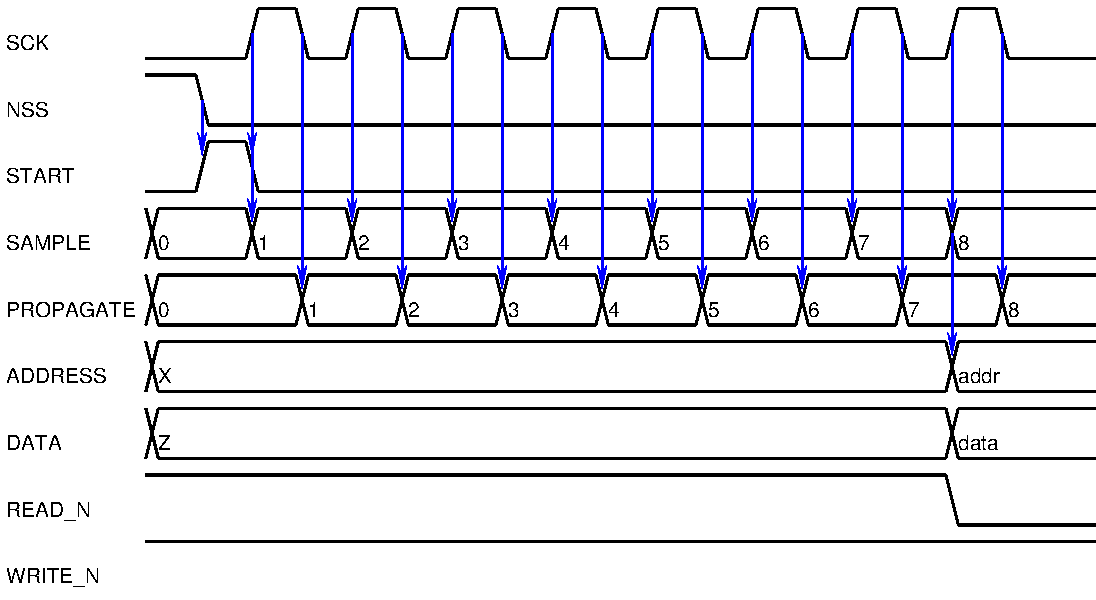
\includegraphics[scale=0.7]{figure/spi_ctl-timing/read-byte1} \\
(a) \\
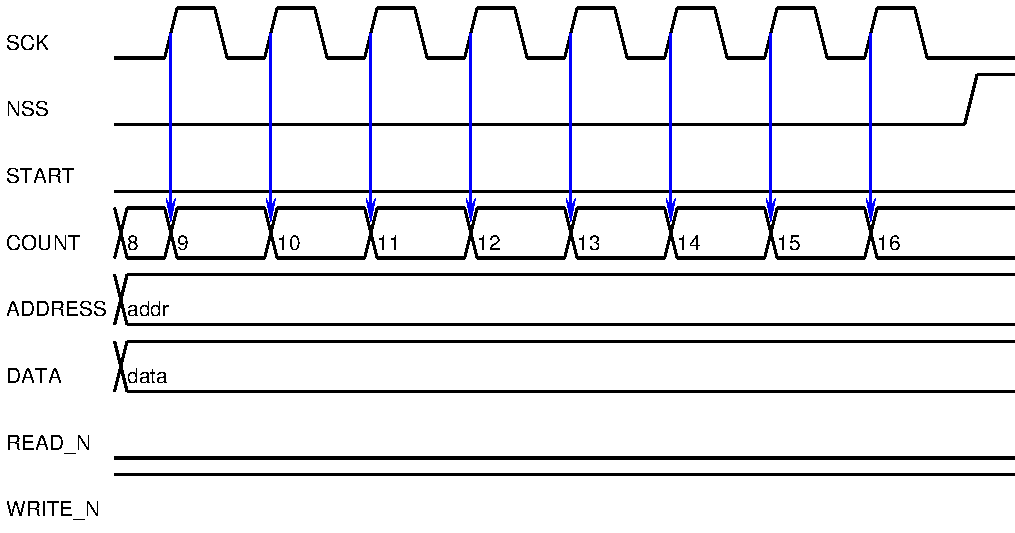
\includegraphics[scale=0.7]{figure/spi_ctl-timing/read-byte2} \\
(b)
\caption{Timing diagram of SPI read cycle.
Part (a) is the first 8-bits and part (b) is the second
8-bits continuing from (a).
Notice in part (a) where the ADDRESS is set and READ\_N becomes active (low).
The data is not immediately read but instead it is delayed until
the negative edge of the SCK.
This is necessary for device such as RAM chips which may not produce
valid data until a short time delay.}
\label{fig:spi_read}
\end{figure}

\begin{figure}
\center
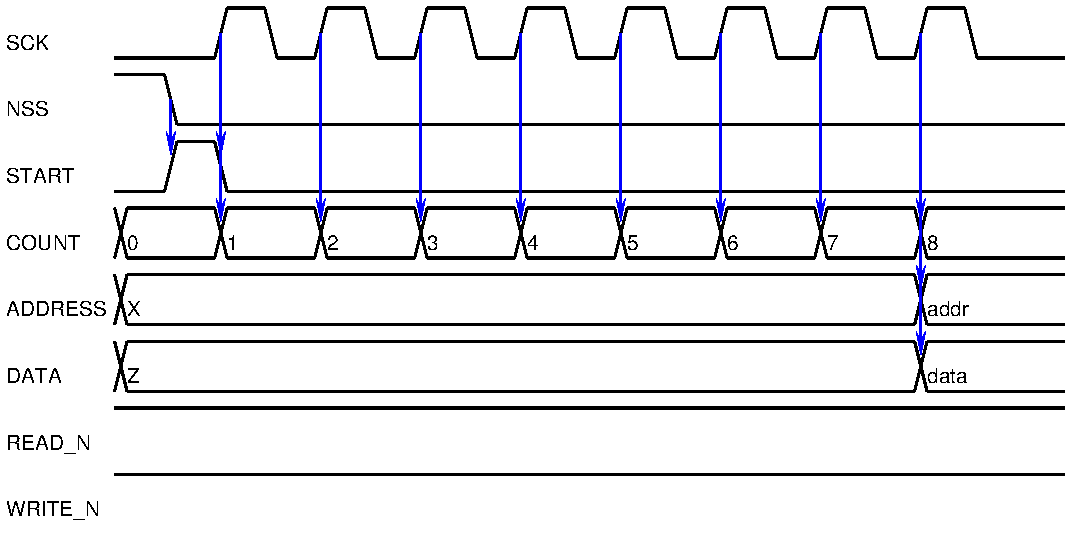
\includegraphics[scale=0.7]{figure/spi_ctl-timing/write-byte1} \\
(a) \\
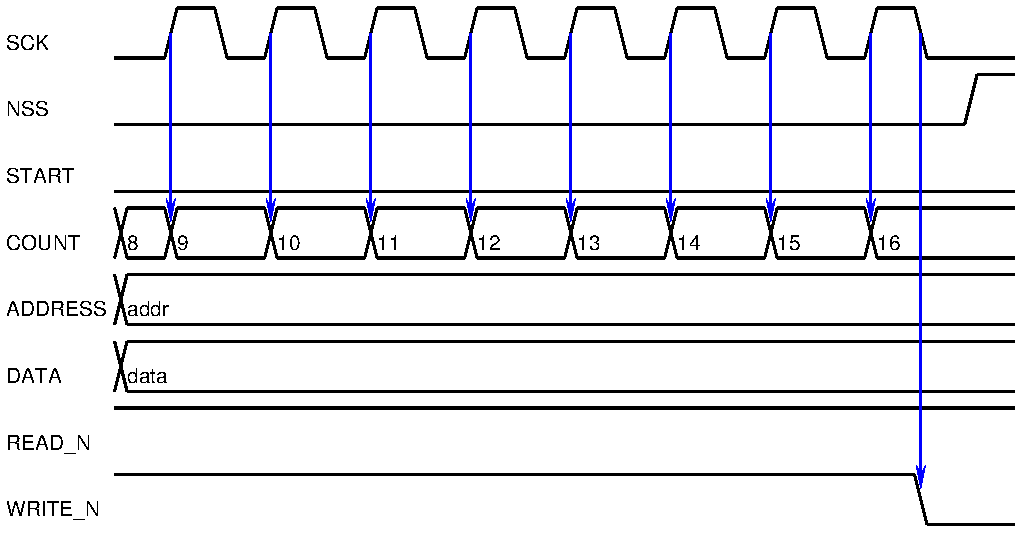
\includegraphics[scale=0.7]{figure/spi_ctl-timing/write-byte2} \\
(b)
\caption{Timing diagram of SPI write cycle.
Part (a) is the first 8-bits and part (b) is the second
continuing from (a).
A write is not initiated until the end of the
second byte because it has to read this byte entirely before it can be written.}
\label{fig:spi_write}
\end{figure}

When values are read or written to the bus they must be held for
some amount of time.
In this implementation this is accomplished by controlling the
pulse width from the end of the 16'th \verb+sck+ edge and the positive
edge of \verb+nss+ (going disabled).
Since the clock speed of the SPI is on the order of kHz and the
clock inside the CPLD is on the order of MHz there should be plenty
of time for any memory timings or other operations to be done.

% }}}

% {{{ Bus Interface
\section{Bus Interface}

% }}}

% {{{ References
\clearpage

\pagebreak
\renewcommand*{\refname}{\vspace{-8mm}}
\section{References}
%\bibliographystyle{ieeetr}
\bibliographystyle{plain}
\bibliography{references}
% }}}

\end{document}

% vim:foldmethod=marker

